\documentclass[letterpaper,sansserif,tightsqueeze]{rpg-module}

\usepackage{parskip}                                                            % Add spacing between paras instead of indents
\usepackage[font=bf]{caption}
\usepackage{hyperref}

\title{Excavated Thaumaturgy}

% Compress title spacing compared to default

\addtolength{\topmargin}{-0.3cm}
\addtolength{\textheight}{0.7cm}

\begin{document}

\twocolumn

\title{Excavated Thaumaturgy}

\subtitle{Optional Rules and Miscellaneous Artifacts}

\coverimage{weapons.png}

\abstract{$\ll$Abstract in construction$\gg$.}


\maketitle

\vspace{0.5cm}
\part*{Optional Rules for Combat}
\vspace{0.5cm}

\begin{center}
	
\includegraphics[width = 0.3\linewidth]{dead.png}
\end{center}
\section{Bleeding out}
\textit{This rule is intended to add an unpredictable element to dying in battle.}

Instead of dying immediately when a damaging effect causes your HP to go to 0 or lower, you start bleeding out:
\begin{itemize}
	\item You immediately gain a pool of \textit{bleed out points}, this pool starts at 0.
	\item You have to stay prone and cannot act except for moving 5 feet.
	\item The GM rolls a d6 whenever you would normally act and increases your bleed out points by the rolled result without disclosing the either the roll or the total.
	\item The GM rolls another d6 and adds the result to the PC's total any time the PC is hit by a damaging effect.
	\item When the total is equal to or exceeds the PC's Constution score, the PC has bled out and dies.
\end{itemize}
\textbf{Applying pressure:} Other players can stop the bleeding by spending their turn taking care of the bleeding PC, the PC then becomes \textit{Stabilized}, this state is negated when the PC takes damage.

\textbf{Healing:} A downed PC can only be healed - magically or non-magically - when he or she has been stabilized. The bleed out pool is reset once the PC is healed, the bleed out score does not affect the amount of HP restored.
\vspace{0.5cm}
\section{0-level spells}
\textit{This optional rule can be used to make the magic user ever so slightly more mischievous. Copied from \href{http://saveordie.info/?p=90}{saveordie.info}}

The Cantrip is a tiny spell created by practicing students of the magical arts during their apprenticeship and while a minor dweomer they still have some uses to the adventuring Magic-User. Elves do not obtain cantrips at first level as they don’t learn such in their youth, though a friendly Magic User may teach them at a later date.

Cantrips are cast like normal spells, only the number that a Magic User may keep in their mind at one time is equal to their Magic User level plus their Intelligence bonus. Therefore, a 1st level MU with a 16 Intelligence (+2) would start with 3 cantrips, while a 6th level MU with a 13 Intelligence (+1) would be capable of casting up to 7. As with other spells, cantrips may be memorized multiple times as desired. If a caster wished, 4 cantrips could be memorized in lieu of a 1st level spell.

A 1st level Magic User starts out with 1d4 + Intelligence modifier of cantrips known and written in their spell book. Others may be obtained during adventures just as any other spell.
\newpage
\textbf{Spells:}
\begin{itemize}
	\item Anatomics
	\item Bug
	\item Clean
	\item Enrich
	\item Exterminate
	\item Firefinger
	\item Hairy
	\item Haunting
	\item Legerdemain
	\item Repair
	\item Temperature
	\item Transmogrify
	\item Unseen Hand
\end{itemize}
\textbf{Anatomics (Evocation)}\\
Level: 0\\
Area of Effect: One person\\
Duration: 1 action\\
Saving Throw?: None
	
When this cantrip is cast, the subject will involuntarily emit a body noise or reaction of the casters choosing. Such simple reactions can be a belch, blink, nod, yawn, etc; but nothing sophisticated
	
\textbf{Bug (Summoning)}\\
Area of Effect: 10 feet\\
Duration: Permanent\\
Saving Throw?: None

When this cantrip is used, the caster summons an insect from someplace — where is of no importance, for the creature appears in seconds. The bug will appear in whatever spot the caster is gazing at, up to a 10 foot distance from him or her. The bug is, of course, annoyed, and it is 90\% likely to sting or bite (if possible) any living creature it finds itself upon. (This will certainly cause the subject to react violently if it would otherwise be so affected by such).
	
\textbf{Clean (Abjuration)}\\
Area of Effect: 4 sq. yards\\
Duration: Permanent\\
Saving Throw?: None
	
This cantrip enables the caster to remove heavy soil, dirt, and like foreign objects from floors, walls, dishes, windows, clothing, etc. The subject surfaces are then spotless, but care must be taken in removal of pigments and the like, so usually only one type of material will be treated in a single application. The reverse of this cantrip dirties and befouls any surface equal to the area of effect.
	
\textbf{Enrich (Enchantment)}\\
Area of Effect: One object\\
Duration: Up to 6 turns\\
Saving Throw?: None

This cantrip enables the caster to give the subject a superior or better or different aspect of its to the senses; be they sight, smell, sound, touch or taste. Thus, mush can be made to taste as if it were lobster bisque, but the dweomer will not actually affect quality or wholesomeness. It can also be used to restore faded hues or to tinge those already colored with a different hue. A rough canvas garment can be made to feel like silk or velvet. A rotten egg can smell like fresh daisies, and a irritating sound can be made to sound like a canary’s song. However, the cantrip may only effect one sense per casting.
	
\textbf{Exterminate (Abjuration)}\\
Area of Effect: One small creature\\
Duration: Permanent\\
Saving Throw?: See below

When this cantrip is used, the caster may kill a small pest such as a fly, mouse, (non-giant) rat, beetle, or the like. It is useful for indoor and outdoor applications. If the subject is very small, an area of up to 1/2 cubic foot can be rid of pests. This cantrip is effective against magical creations and normal-sized creatures magically shrunk to insect-size, with a saving throw applicable to negate. The dweomer however has no effect on polymorphed creatures and similarly enchanted beings.
	
\textbf{Firefinger (Alteration)}\\
Area of Effect: 1/3' line\\
Duration: 1 round\\
Saving Throw?: None
	
The firefinger cantrip enables the caster to cause a jet of flame up to one-half foot in length to shoot forth from his or her finger. The flame is very hot and will ignite combustible materials such as parchment, twigs, kindling, and the like without difficulty, providing the materials are relatively dry. The flame persists for up to 1 round.
The reverse of this Cantrip extinguishes a small flame such as used in a lantern or candle. A torch is too large a flame to be effected with this cantrip.
	
\textbf{Hairy (Alteration)}\\
Area of Effect: One object\\
Duration: Permanent\\
Saving Throw?: None
	
While this cantrip is not actually one of the standard useful ones which apprentices reverse for mischievousness, it is one which is generally used for no good purpose. It causes hair, fur, or hairlike growth to thicken and lengthen. Thus, a head of hair, a peach, a beard, a cat, or whatever could be affected. The growth will cause the subject material to increase from 2-12 inches in length. The subject material must be trimmed or cut to remove the cantrip’s effect. This cantrip can be reversed to shorten growth or effectively shave, but since the effect on short material (growth under 1 inch in length) is complete absence of growth for 2-12 days, it is not often used.
	
\textbf{Haunting (Illusion)}\\
Area of Effect: Special\\
Duration: See below\\
Saving Throw?: Yes

This cantrip creates the illusion of any number of ghostly sounds such as a faint groan, creak, footfalls, etc. Naturally, those creatures within hearing distance are allowed a saving throw versus spell, and if it succeeds, the individual will hear no such noise. The sound only lasts from 1-20+ Magic User’s level in seconds.

\textbf{Legerdemain (Illusion)}\\
Area of Effect: One small item\\
Duration: 1 round\\
Saving Throw?: None
	
This cantrip enables the caster to secret or cause to appear a small object in his hand without seeming to do so. The item created to appear from nowhere is illusory, and will disappear in 1 round.
	
\textbf{Repair (Alteration)}\\
Area of Effect: One object\\
Duration: Permanent\\
Saving Throw?: None
	
This cantrip repairs small breaks in objects. It will weld a broken ring, chain link, medallion or ripped material, providing but one break exists. Ceramic or wooden objects with multiple breaks can be invisibly rejoined to be as strong as new. A hole in a leather sack or wineskin is completely healed over by a Repair cantrip. This cantrip will not repair magic items of any kind.
	
\textbf{Temperature (Evocation)}\\
Area of Effect: 1' cube\\
Duration: Special\\
Saving Throw?: none
	
A cantrip of this nature allows the caster to cause non-living liquid or solid material to become about 40°F. warmer or cooler than it was, subject to a minimum temperature of freezing. The warming or chilling effect lasts for but an instant, after which the subject returns slowly back to ambient temperature as normal for the current climate.
	
\textbf{Transmogrify (Alteration)}\\
Area of Effect: One creature/item\\
Duration: See below\\
Saving Throw?: See below
	
By means of a transmogrify cantrip, the caster alters one small object to another, although the change must be within the same kingdom, and only animal and vegetable objects are affected. Thus, a piece of parchment can be changed to a brightly colored cloth square, then the cloth can be changed to a rose by another use of the cantrip. Likewise, a bird can be changed into a bat, the bat to a flying squirrel by another use of the same type of cantrip, and so forth. Each alteration requires a transmogrify cantrip. The cantrip will not cause more than a 50\% increase or decrease in size/volume, and the effect will last for a base time of 1 turn. If the change is radical, then the time will be reduced accordingly; i.e., changing a dead object to a live one is a radical change and will last only 1 round. On the other hand, a very slight alteration such as color change or the like will last for 1 or more days. A saving throw against this magic does not apply as long as small, animal-intelligence, non-magical creatures of normal sort are concerned.
	
\textbf{Unseen Hand (Conjuration)}\\
Area of Effect: One creature/item\\
Duration: 1 action\\
Saving Throw?: Save vs. Magic to avoid a 1 round distraction.
	
By means of this cantrip, the caster causes an unseen hand to perform simple actions such as open/close a door, lift a small object and carry it (1 lb limit) within 10 feet radius of the caster, and poke or pinch a target as desired.
If this cantrip is used on a spellcaster, the target must make a saving throw vs. magic, with success meaning that the target is not distracted. Failure causes a 1 round distraction and may interrupt spell casting at DM’s discretion.
\newpage

\vspace{0.5cm}
\part*{Cursed Artifacts}
\vspace{0.5cm}

\begin{center}
	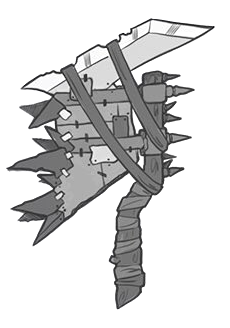
\includegraphics[width = 0.5\linewidth]{Garthruks_axe.png}
\end{center}
\section{The Axe of Garthruk}
\textit{A blackened axe made with crude green metal. It angrily shakes when approached.}

Garthruk the Orc Chief is captured within the axe. He wants to challenge the great and mighty, and escape his metal prison.

Abilities:
\begin{itemize}
	\item \textbf{Orcish Strength:} The wielder's muscles bulge and he suddenly can perform orcish feats of strength.
	\item \textbf{Possession:} When triggered, Garthruk will try to possess the wielder. Save against Paralysis or be possessed for 3d6 minutes by a raging Orc. Possession occurs when one of the following conditions is met:
	\begin{itemize}
		\item Attempting to get rid of the axe (automatic possession, no save allowed).
		\item Evading a mighty foe.
		\item Failing to protect your honor.
	\end{itemize}
	\item \textbf{Corruption:} Every failed save gives the wielder an Orc point. After the wielder reached his Orc threshold - 2d6 rolled in secret by the GM after touching the axe - the wielder will count as being an Orc instead of his/her former race.
\end{itemize}
Stages: 
\begin{itemize}
	\item \textbf{Stage 1 (1 Orc point}:) The wielder's face becomes cruder ever so slightly. His/her speech becomes rougher. 
	\item \textbf{Stage 2 (Orc threshold/2, rounded down):} The wielder becomes a half-Orc.
	\item \textbf{Stage 3: (Orc threshold):} The wielder is now a full-fledged Orc.
\end{itemize}

\end{document}
